\documentclass[border=6pt]{standalone}
% Shared preamble of every figure (included by each fig*.tex)
\usepackage{fontspec}
\setmainfont{DejaVu Sans}
\setmonofont{DejaVu Sans Mono}
\usepackage{amsmath,amssymb}
\usepackage{tikz}
\usetikzlibrary{positioning,arrows.meta,fit,calc,decorations.pathreplacing,shapes.geometric,backgrounds}
\definecolor{cdata}{HTML}{4C78A8}
\definecolor{cmodel}{HTML}{F58518}
\definecolor{chead}{HTML}{54A24B}
\definecolor{cgold}{HTML}{E45756}
\definecolor{cgrey}{HTML}{9D9D9D}
\definecolor{cfull}{HTML}{B279A2}
\tikzset{
  box/.style={draw, rounded corners=2pt, align=center, inner sep=4pt, font=\small, minimum height=8mm},
  data/.style={box, fill=cdata!15, draw=cdata!80!black},
  model/.style={box, fill=cmodel!18, draw=cmodel!80!black},
  head/.style={box, fill=chead!18, draw=chead!70!black},
  note/.style={font=\footnotesize, align=center, text=black!70},
  arr/.style={-{Stealth[length=2.2mm]}, thick, black!70},
}

\tikzset{lay/.style={box, minimum width=34mm, font=\footnotesize}}
\begin{document}
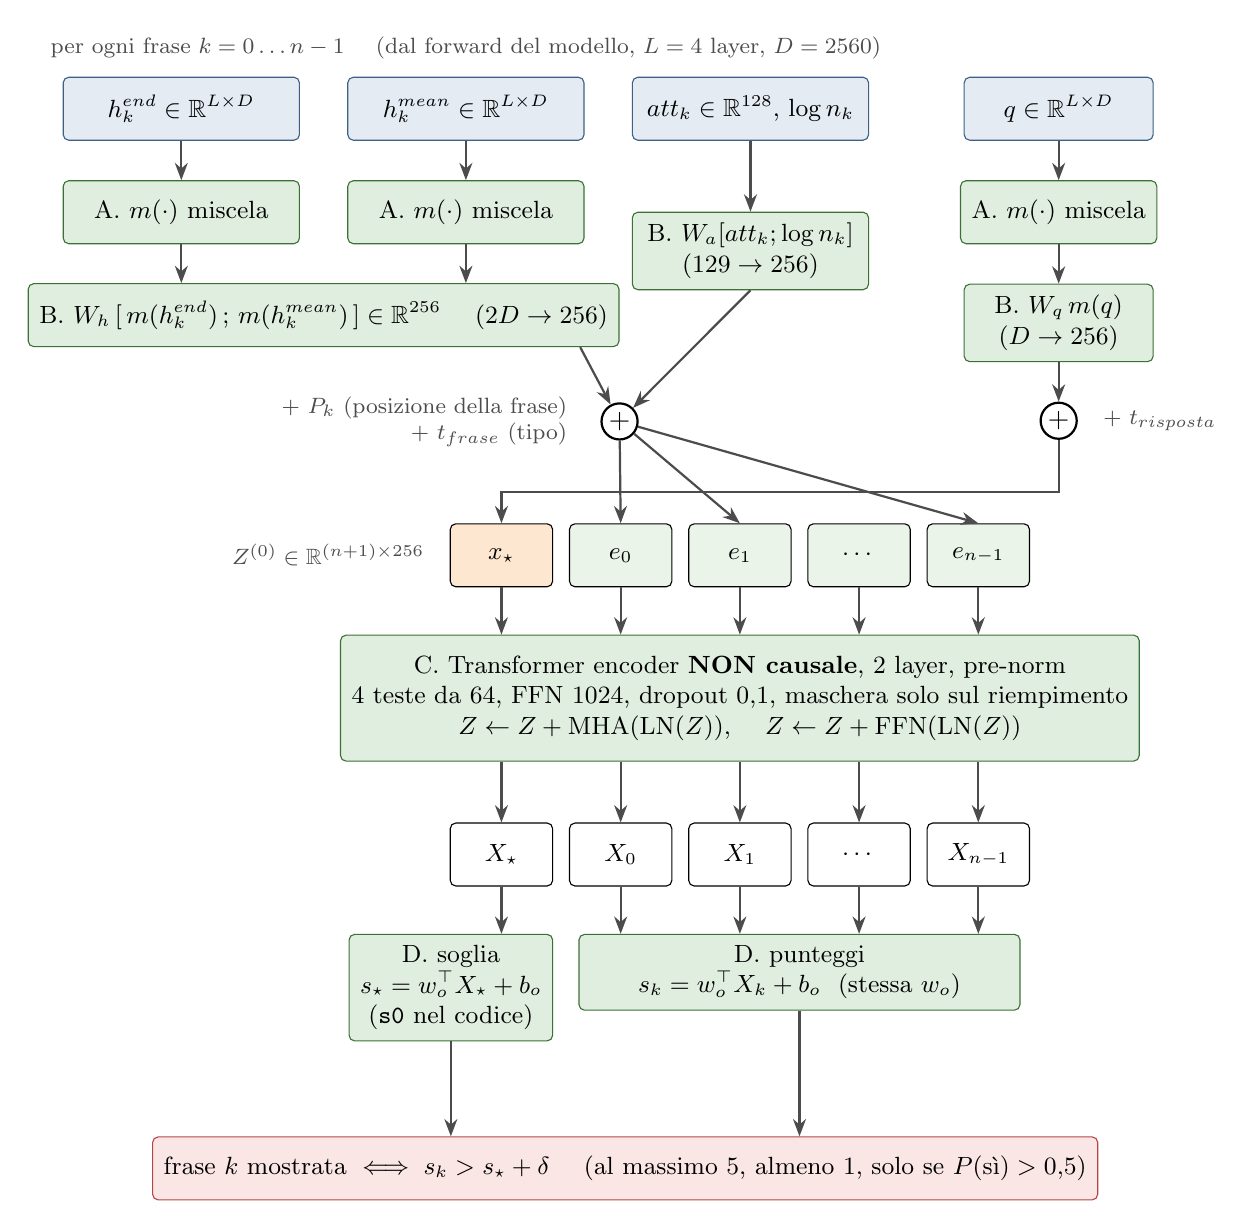
\begin{tikzpicture}[node distance=5mm and 6mm]
% inputs
\node[data, minimum width=30mm] (hend) {$h^{end}_k \in \mathbb{R}^{L\times D}$};
\node[data, minimum width=30mm, right=of hend] (hmean) {$h^{mean}_k \in \mathbb{R}^{L\times D}$};
\node[data, minimum width=30mm, right=of hmean] (att) {$att_k \in \mathbb{R}^{128}$, $\log n_k$};
\node[data, minimum width=24mm, right=12mm of att] (q) {$q \in \mathbb{R}^{L\times D}$};
\node[note, above=1mm of hmean] {per ogni frase $k=0\dots n-1$ \quad (dal forward del modello, $L=4$ layer, $D=2560$)};
% A: mix
\node[head, below=of hend, minimum width=30mm] (mixe) {A. $m(\cdot)$ miscela};
\node[head, below=of hmean, minimum width=30mm] (mixm) {A. $m(\cdot)$ miscela};
\node[head, below=of q, minimum width=24mm] (mixq) {A. $m(\cdot)$ miscela};
% B: projections
\node[head, below=9mm of $(mixe)!0.5!(mixm)$, minimum width=66mm] (wh) {B. $W_h\,[\,m(h^{end}_k)\,;\,m(h^{mean}_k)\,] \in \mathbb{R}^{256}$ \quad ($2D \to 256$)};
\node[head, below=9mm of att, minimum width=30mm] (wa) {B. $W_a [att_k ; \log n_k]$\\($129 \to 256$)};
\node[head, below=of mixq, minimum width=24mm] (wq) {B. $W_q\, m(q)$\\($D \to 256$)};
\node[circle, draw, thick, inner sep=1pt, below=7mm of wh.south east] (plus) {$+$};
\node[note, left=3mm of plus, align=right] {$+\ P_k$ (posizione della frase)\\$+\ t_{frase}$ (tipo)};
\node[circle, draw, thick, inner sep=1pt, below=5mm of wq] (plusq) {$+$};
\node[note, right=2mm of plusq] {$+\ t_{risposta}$};
\draw[arr] (hend) -- (mixe); \draw[arr] (hmean) -- (mixm); \draw[arr] (q) -- (mixq);
\draw[arr] (mixe) -- (mixe|-wh.north); \draw[arr] (mixm) -- (mixm|-wh.north);
\draw[arr] (att) -- (wa); \draw[arr] (mixq) -- (wq);
\draw[arr] (wh.south east) ++(-5mm,0) -- (plus); \draw[arr] (wa.south) -- (plus);
\draw[arr] (wq) -- (plusq);
% sequence [x0, e_0 ... e_{n-1}]
\node[box, minimum width=13mm, fill=cmodel!20] (z0) at ($(plus)+(-15mm,-17mm)$) {$x_\star$};
\node[box, minimum width=13mm, fill=chead!12, right=2mm of z0] (z1) {$e_0$};
\node[box, minimum width=13mm, fill=chead!12, right=2mm of z1] (z2) {$e_1$};
\node[box, minimum width=13mm, fill=chead!12, right=2mm of z2] (z3) {$\cdots$};
\node[box, minimum width=13mm, fill=chead!12, right=2mm of z3] (z4) {$e_{n-1}$};
\node[note, left=2mm of z0] {$Z^{(0)} \in \mathbb{R}^{(n+1)\times 256}$};
\draw[arr] (plus) -- (z1.north); \draw[arr] (plus) -- (z2.north); \draw[arr] (plus) -- (z4.north);
\draw[arr] (plusq.south) |- ($(z0.north)+(0,4mm)$) -- (z0.north);
% C: encoder
\node[head, minimum width=86mm, minimum height=16mm, anchor=north] (enc) at ($(z2.south)+(0,-6mm)$) {C. Transformer encoder \textbf{NON causale}, 2 layer, pre-norm\\4 teste da 64, FFN 1024, dropout 0,1, maschera solo sul riempimento\\$Z \leftarrow Z + \mathrm{MHA}(\mathrm{LN}(Z))$, \quad $Z \leftarrow Z + \mathrm{FFN}(\mathrm{LN}(Z))$};
\foreach \i in {0,...,4}{ \draw[arr] (z\i.south) -- (z\i.south|-enc.north); }
% D: outputs
\node[box, minimum width=13mm] (o0) at ($(z0)+(0,-38mm)$) {$X_\star$};
\node[box, minimum width=13mm] (o1) at ($(z1)+(0,-38mm)$) {$X_0$};
\node[box, minimum width=13mm] (o2) at ($(z2)+(0,-38mm)$) {$X_1$};
\node[box, minimum width=13mm] (o3) at ($(z3)+(0,-38mm)$) {$\cdots$};
\node[box, minimum width=13mm] (o4) at ($(z4)+(0,-38mm)$) {$X_{n-1}$};
\foreach \i in {0,...,4}{ \draw[arr] (o\i.north|-enc.south) -- (o\i.north); }
\node[head, anchor=north east] (s0) at ($(o0.south east)+(0,-6mm)$) {D. soglia\\$s_\star = w_o^\top X_\star + b_o$\\(\texttt{s0} nel codice)};
\node[head, minimum width=56mm, anchor=north] (sk) at ($($(o1.south west)!0.5!(o4.south east)$)+(0,-6mm)$) {D. punteggi\\$s_k = w_o^\top X_k + b_o$ \ (stessa $w_o$)};
\draw[arr] (o0.south) -- (o0.south|-s0.north);
\foreach \i in {1,...,4}{ \draw[arr] (o\i.south) -- (o\i.south|-sk.north); }
\node[box, fill=cgold!15, draw=cgold!80!black, anchor=north, minimum width=110mm] (sel) at ($($(s0.south)!0.5!(sk.south)$)+(0,-14mm)$) {frase $k$ mostrata $\iff s_k > s_\star + \delta$ \quad (al massimo 5, almeno 1, solo se $P(\text{sì}) > 0{,}5$)};
\draw[arr] (s0.south) -- (s0.south|-sel.north); \draw[arr] (sk.south) -- (sk.south|-sel.north);
\end{tikzpicture}
\end{document}
